\chapter{Conceitos gerais e revisão da literatura}
Neste capítulo deve ser proporcionado o estado da arte / referencial teórico
sobre o tema a que se refere o estudo. Um bom pesquisador não deve repetir
trabalhos já concluídos ou que já estão em andamento. Por isso esta sessão é
onde o autor demonstra até onde vai a pesquisa atual no campo de estudos em
questão e estabelece as bases sobre as quais desenvolverá o estudo proposto. A
seguir são mostrados alguns exemplos de como deve-se inserir as figuras e
tabelas. A Figura \ref{fig:exemplo} mostra um exemplo de como inserir uma
figura no texto. A Tabela \ref{tb:exemplo} mostra o exemplo de como uma tabela
deve ser inserida.  Voce pode referenciar capítulos e seções adicionando labels
à elas. Por exemplo, descrevemos a introdução no Capítulo
\ref{chp:introduction}.

\begin{figure}[!htb]
    \centering
    \caption{Exemplo de como inserir Figura}
    
\includegraphics[width=0.45\textwidth]{images/figura.png}
    {\footnotesize Fonte: Inserir fonte conforme padrão ABNT.}
    \label{fig:exemplo}
\end{figure}

%Altere o numero junto ao 'width' para acertar o tamanho da figura. Coloque
%numeros maior que 0 e até 1


%Voce pode forcar a troca de pagina da seguinte forma:
\newpage

%Ao retirar figura de um site.
%\begin{figure}[!htb]
%    \centering
%    \caption{Exemplo de como inserir Figura retirado de um site - Arduino Uno}
%    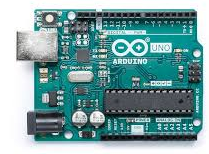
\includegraphics[width=0.35\textwidth]{images/uno.png}

%    {\footnotesize Fonte: Página oficial do Arduino\protect\footnotemark}
%    \label{fig:arduino_uno}
%\end{figure}
%\footnotetext{Disponível em: <https://www.arduino.cc/en/Main/ArduinoBoardUno>. Acesso em ago. 1999.}

\begin{table}[htb]
\caption{Modelo de como as tabelas devem ser inseridas no texto}
\label{tb:exemplo}
\centering
\begin{tabular}{|l|c|r|r|} %left, center, right. Você pode mudar isso
\hline
Índice  & Coluna 1 & Coluna 2 & Coluna 3 \\
\hline
Linha 1 &          &          &          \\
Linha 2 &          &          &          \\
Linha 3 &          &          &          \\
\hline
\end{tabular}
\end{table}
%Para manter a sanidade, recomenda-se deixar sempre os '&' alinhados em todas
%as linhas e colunas

\section{Tecnologias}
Esse capítulo apresenta as tecnologias usadas no desenvolvimento do sistema. Como linguagem de programação, foi utilizado o PHP, acessado via servidor Nginx, com o auxílio do framework Laravel. Para a base de dados, foi utilizado sistema de gerenciador de banco de dados MariaDB. Para orquestrar todos os serviços necessários para subir a aplicação, foi utilizado o Docker.

\subsection{PHP}
Desde sua criação em 1994, a linguagem PHP (Hypertext Preprocessor ou preprocessador de hypertexto, no português), vem sendo amplamente utilizada na web. Mais de 70\% dos sites da web usam PHP no lado do servidor \citep{w3techs}.

    A linguagem PHP permite que se trabalhe tanto com servidores windows como servidores linux, a sua evolução permititu que a linguagem abordasse paradigmas estruturados e orientadado a objetos, e comporta diversos bancos de dados, e vem recebendo atualizações constantes, sendo uma lingugem que pode ser tranquilamente utilizada em novos projetos \citep{phpdocs}.
    
\subsection{Laravel}
    Laravel é um framework que traz consigo diversas funcionalidades através das suas bibliotecas consolidadas, que vem agregadas ao seu núcleo. Lançado sua primeira versão em 2011, hoje se encontra na versão 9, acompanhando e explorando as novas funcioncionalidades das versões mais atuais do php \citep{laradocs}.
    
        O framework hoje conta com 70 mil estrelas no github, o que indica que é um framework bastante conhecido e consolidado no mercado. Atende tanto pequenos quanto grandes projetos, sempre utilizando os padrões mais modernos da linguagem \citep{lararepo}
        
\subsection{Laravel Auditing}
    Laravel Auditing, é uma biblitoeca feito para o laravel framework, com o intuito de permitir salvar as mudanças e alterações executadas nas classes de modelo do laravel. Sua configuração padrão permite que registre e recupere os históricos de alterações a partir de uma base de dados, mas também permite que realize a integração com outros meios de logs, como salvar em arquivos ou criar seu próprio driver, para atender a uma necessidade específica \citep{auditdocs}.
    

\subsection{MariaDB}
    MariaDB é um sistema gerenciador de banco de dados relacional, que está a mais de 20 anos no mercado.  Sendo um software de codigo aberto, recebe contantes contribuições de comunidades de desenvolvedores que o utilizam, inclusive patches de segurança, tendo esse como um dos principais motivos para utilizá-lo no projeto \citep{mariadbdocs}.
    
\subsection{Nginx}
    Escrito por Igor Sysoev, o Nginx é um servidor de proxy reverso HTTP, proxy de servidor de e-mail e um proxy generico de TCP/UDP. Uma de suas características é a possibilidade de configurá-lo em servidores distintos, suportando servidores tanto windows como linux \citep{nginxdocs}.

    Oferece um alto desempenho de conexões, sendo seu uso recomendável para aplicações que exigem muitas requisiçoes, ou seja, é escalável e de código aberto.
    
\subsection{Docker}

    Docker, tecnologia que divide a aplicação em pequenos containers, tendo cada uma a sua configuração, distinta umas das outras. Permite a entrega rápida de software, e a reprodução do mesmo ambinte tanto pra desenvolvimento quanto homologação e produção \citep{dockerdocs}. 